\newpage

\titleformat % design des titres des chapitres
{\chapter}
[display]
{\centering\normalfont\Large\scshape\bfseries}
{\rule[3pt]{0.15\linewidth}{3pt}\quad\chaptertitlename~\thechapter\quad \rule[3pt] {0.15\linewidth}{3pt}}
{0\baselineskip}%espace vertical entre chapitre et nom du chapitre
{\rule{\linewidth}{0.5pt}\break\Huge}
[\vspace{-0.5\baselineskip}\rule{\linewidth}{0.5pt}\vspace{0\baselineskip}]

\let\clearpage\relax% Stop LaTeX from going to a new page; and
\vspace*{5.5cm}%

\chapter{Etude Technique}
Dans ce chapitre, je vais présenter les outils de développement adoptés ainsi que
l’architecture technique et applicative du projet

\newpage

\section{Architecture Logique :}
Pour le développement de la solution j'ai utilisé Microsoft Power Platform qui permet la réalisation d'application web/mobile en low-code voire no-code. 
\\ \\
Cette methodologie de low code represente la principale puissance de cette derniere car elle permet de realiser des projets web sans avoir beaucoup de connaisance technique dans le monde du developpement.
\\

Les principaux composant de microsoft power platform sont:

\begin{itemize}
  \item Power Apps 
  \item Power BI 
  \item Power Automate
  \item Power Virtual Agents
\end{itemize}

\section{Power Platform :}

\subsection{Power Apps: }
\vspace{0.5cm}

\begin{wrapfigure}{l}{0.4\textwidth}
  \begin{center}
    
\includegraphics[width=0.4\textwidth]{Rapport de stage PFE chez DXC/figures/power_apps.png}
  \end{center}
\end{wrapfigure}

Power Apps est une suite d’applications, de services, de connecteurs et une plateforme de données qui fournissent un environnement de développement rapide dans le but de concevoir des applications personnalisées et adaptées à vos besoins métier.
\\
\\
Les applications créées à l’aide de Power Apps fournissent une logique métier et des capacités de flux de travail enrichies pour transformer vos opérations d’entreprise manuels en processus numériques et automatisés. De plus, les applications conçues à l’aide de Power Apps ont une conception réactive et elles peuvent fonctionner de manière transparente dans un navigateur ou sur des appareils mobiles (téléphone ou tablette).

\newpage
\subsection{Power Automate: }

\begin{wrapfigure}{l}{0.4\textwidth}
  \begin{center}
    
\includegraphics[width=0.4\textwidth]{Rapport de stage PFE chez DXC/figures/power_automate.png}
  \end{center}
\end{wrapfigure}

Power automate est un puissant outils d'automatisation qui permet de :
\begin{itemize}
  \item Automatiser les processus d’entreprise
  \item envoyer des rappels automatiques sur les tâches en retard ;
  \item Se connecter à plus de 500 sources de données ou à toute API accessible au public
\end{itemize}
\\ 
\\
Tout cela sans avoir conaissance technique specifique, n'importe quelle utilisateur pourrait créer ainsi que manipuler des processus automatisée en utilisant la plateforme Power Automate qui represente elle aussi un environement low-code/no-code

\subsection{Power BI: }

\begin{wrapfigure}{l}{0.4\textwidth}
  \begin{center}
    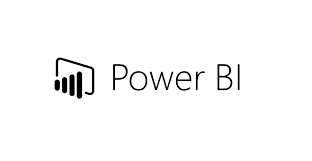
\includegraphics[width=0.4\textwidth]{Rapport de stage PFE chez DXC/figures/power_bi.png}
  \end{center}
\end{wrapfigure}

Power BI est un ensemble de services logiciels, d’applications et de connecteurs qui œuvrent ensemble pour transformer des sources de données disparates en informations visuelles immersives et interactives. 
\\
Vos données peuvent être sous forme de feuille de calcul Excel ou de collection d’entrepôts de données hybrides locaux ou sur le cloud. Power BI vous permet de vous connecter facilement à vos sources de données, de visualiser et de découvrir ce qui est important, et de partager ces informations avec qui vous voulez.

%
%Power BI est constitué de plusieurs éléments qui fonctionnent ensemble, dont ces trois éléments de base :
%\begin{itemize}
  %\item Une application de bureau Windows appelée Power BI Desktop.
  %\item Un service SaaS (Software as a Service) en ligne appelé service Power BI.
 % \item Des applications mobiles Power BI pour des appareils Windows, iOS et Android.
%\end{itemize}
%

\subsection{Power virtual agent :}

\begin{wrapfigure}{l}{0.4\textwidth}
  \begin{center}
    
\includegraphics[width=0.4\textwidth]{Rapport de stage PFE chez DXC/figures/power_virtual_agent.png}
  \end{center}
\end{wrapfigure}

Power Virtual Agents vous permet de créer des chatbots puissants qui peuvent répondre aux questions posées par vos clients, d’autres employés ou des visiteurs de votre site Web ou service.

Ces bots peuvent être créés facilement sans avoir besoin de spécialistes des données ou de développeurs. Certaines des façons dont les bots Power Virtual Agents ont été utilisés incluent :

\begin{itemize}
  \item Aide à la vente et problèmes de support
  \item Questions courantes des employés
\end{itemize}

\newpage
\subsection{Dataverse :}

\begin{wrapfigure}{l}{0.4\textwidth}
  \begin{center}
    
\includegraphics[width=0.24\textwidth]{Rapport de stage PFE chez DXC/figures/dataverse.jpg}
  \end{center}
\end{wrapfigure}

Dataverse permet de stocker et de gérer en toute sécurité les données utilisées par les applications métier. Les données à l’intérieur de Dataverse sont stockées dans un ensemble de tables. Une table est un ensemble de lignes (anciennement appelées enregistrements) et de colonnes (anciennement appelées champs / attributs). 
\\
Chaque colonne de la tables est conçue pour stocker un certain type de données, par exemple, le nom, l’âge, le salaire, etc. 
\\
Dataverse comprend un ensemble de base de tables standard qui couvrent des scénarios classiques, mais vous pouvez également créer des tables personnalisées dédiées à votre organisation et les remplir avec des données à l’aide de Power Query. 
\\
Les créateurs d’applications peuvent ensuite utiliser Power Apps pour créer des applications riches qui utilisent ces données.

